\chapter[\glsentrylong{MRI} (\glsentryshort{MRI})]{Magnetic\\Resonance\\Imaging (MRI)}
\vspace{-50ex}
\begin{flushright}
\href{https://www.sciencephoto.com/media/728494/view/normal-brain-mri}{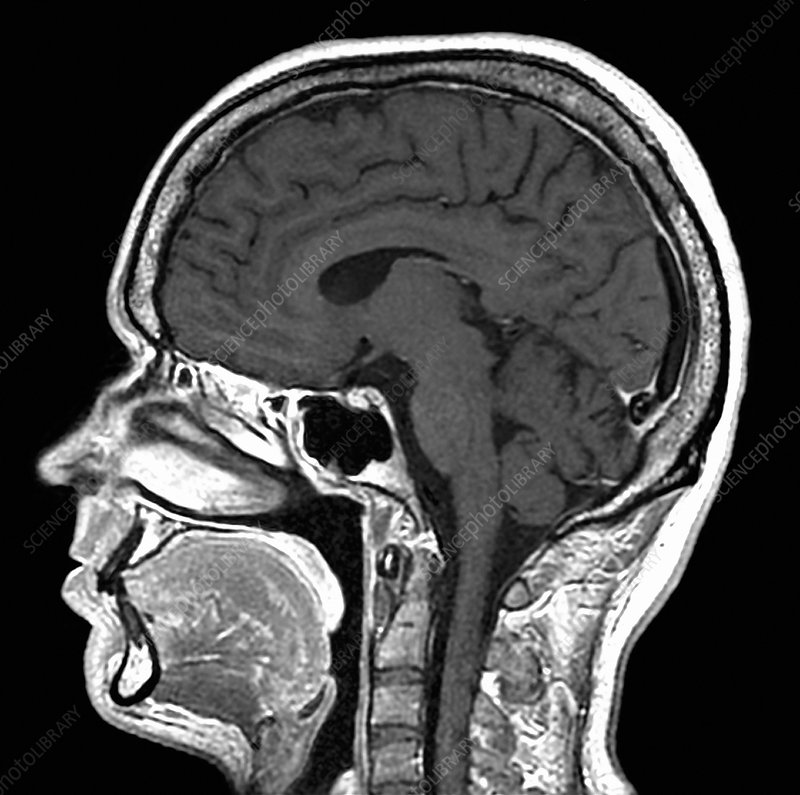
\includegraphics[width=6.5cm]{Normal_brain_MRI}}
\end{flushright}

\section{Clinical applications}
\begin{itemize}
\item \gls{MRI}
  \cite{westbrook2018mri,Wu2022MRI_Physics,thePIRL2018NMR_basics,thePIRL2018SpinEcho,thePIRL2018Fourier,thePIRL2018GRE}
  allows to obtain detailed views of (usually living) samples
  (tissues, organs, and even a complete organism) without irradiate
  them \cite{wikipedia_MRI}.
\end{itemize}

\section{MRI axes}
\begin{itemize}
\item A patient is placed in the bore of the MRI machine to be
  subjected to a $B_0$, a \popup{very strong magnetic field}{In the
    order of Teslas (T). 1 Tesla = 10,000 gauss and the Earth’s
    magnetic field is approx. 0.5 gauss.} parallel to the $Z$-axis.
\end{itemize}
\vspace{-4ex}
\begin{figure}[!b]
  \centering
  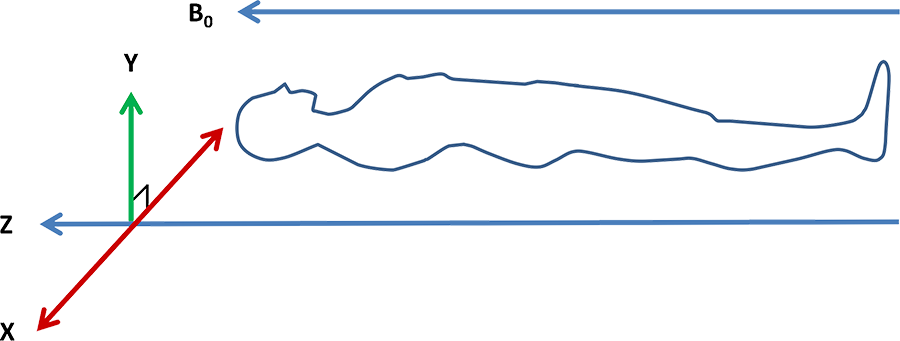
\includegraphics[width=0.8\textwidth]{mri-machine-axes}
  \caption{Axes used in an MRI machine \cite{abdulla2025MRI_machine}.}
  \label{fig:MRI_axes}
\end{figure}

\section{The magnet responsible of $B_0$}
\begin{itemize}
\item $B_0$ is a permanent magnetic field generated by \popup{toroidal
    magnet}{A superconducting electromagnet refigerated with liquid
    helium at -269°C, that can weight several tons.}. A section is
  show in Fig.~\ref{fig:MRI_machine_scheme}.
\end{itemize}
\vspace{-4ex}
\begin{figure}[!b]
  \centering
  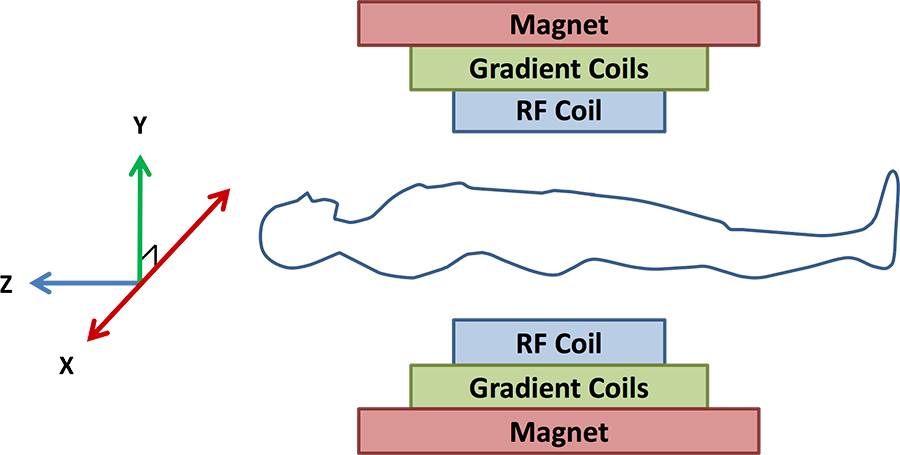
\includegraphics[width=0.7\textwidth]{mri-machine-coils}
  \caption{A schematic section of the MRI machine \cite{abdulla2025MRI_machine}.}
  \label{fig:MRI_machine_scheme}
\end{figure}

\section{Gradient coils}
\begin{itemize}
\item There are three sets of coils orientated in the $X$, $Y$ and $X$
  axes, used to generate a gradient in $B_0$ (see
  Section~\ref{sec:spatial_encoding}).
\item Gradient coils generate a constant variation (gradient) $B_1$ to
  $B_0$ along the $Z$-axis, generating $B_0+B_1$.
\end{itemize}

\section{\glsentrylong{RF} (\glsentryshort{RF}) (body) coil ... and others}
\begin{itemize}
\item In Fig.~\ref{fig:MRI_machine_scheme} the ``body''-coil is shown,
  which is used to image large parts of the patient.
\item This coil transmits and receives \gls{EM} signals.
\item There are other specialized coils (not shown in the figure),
  such as:
  \begin{enumerate}
  \item \textbf{Head coil} (transmit and receive): incorporated into a
    helmet and used for head scans.
  \item Surface (or local) coils (receive only): these are small coils
    applied \popup{as close to the area being imaged as possible}{This
      increases the SNR.} e.g. arm, leg, orbits, lumbar spine coils
    etc.
  \item Arrays of coils that only transmit or receive, and that are
    then combined to improve the SNR.
  \end{enumerate}
\item The RF \cite{wikipedia_RF} coils are \popup{switched on and off
    rapidly}{Forming train of impulses of time-variying period.}, with
  a period of 1 ms or less, and it is this that creates the loud
  noise.
\item The smaller the distance between the coils and the patient, the
  better the strength of the signals, and the higher the \gls{SNR}.
\end{itemize}

\section{Hydrogen nuclei can be considered tiny magnets}
\begin{itemize}
\item Hydrogen nuclei act like tiny \popup{magnets}{A hydrogen nucleus
    contains a single proton so it has a charge of +1. The nucleus
    also has an intrinsic “spin”. Because they have a charge and
    motion they create an electric current and this, in turn, creates
    a magnetic field.} and will be affected by any magnetic field
  applied to them.
\item Hydrogen nuclei are \popup{the most useful atoms}{Any nucleus
    with an odd number of protons can be used (an unpaired proton is
    needed to provide the magnetic moment due to the spin of the
    unpaired proton).} to use in imaging mainly because they form the
  majority of atoms in the body.
\item Most will adopt the low energy state (the direction of $B_0$)
  but a few in the opposite direction (the high energy state),
  creating a net longitudinal magnetization (Mz) in the Z-axis
  direction.
\end{itemize}
\vspace{-4ex}
\begin{figure}[!b]
  \centering
  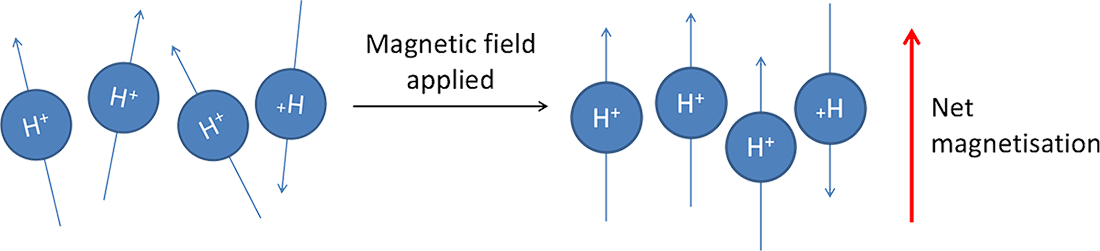
\includegraphics[width=0.7\textwidth]{mri-intro-netmag}
  \caption{Net magnetization under the influence of $B_0$ \cite{abdulla2025MRI_intro}.}
  \label{fig:MRI-intro-netmag}
\end{figure}

\section{Precession}
\begin{itemize}
\item Under the influece of $B_0+B_1$, the hydrogen nuclei precess in the Z-axis.
\item The precession has a characteristic \popup{resonant}{``Larmor''.}
  frequency for each \popup{atom and $B_0+B_1$ intensity}{42 MHz a 1 Tesla
    in the case of hydrogen}.
\end{itemize}
\vspace{-4ex}
\begin{figure}[!b]
  \centering
  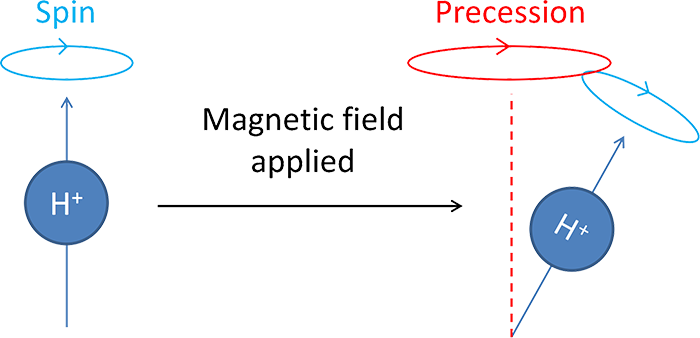
\includegraphics[width=0.7\textwidth]{mri-intro-precession}
  \caption{Nuclei precession \cite{abdulla2025MRI_intro}.}
  \label{fig:MRI-intro-precession}
\end{figure}

\section{Resonance magnetization}
\begin{itemize}
\item When all the nuclei are precessing, an orthogonal to $B_0+B_1$
  ($Z$-axis) time-varying magnetization oscillating at the resonance
  frequency is applied from the RF coil, making the nuclei to resonate
  in the $XY$ plane.
\end{itemize}

\section{Relaxation $T_1$ and $T_2$ times}
\begin{itemize}
\item As soon as $B_1$ is switched off, the transverse magnetization
  begins to disappear and the nuclei relax back to their resting state
  of net longitudinal magnetization. 
\item \popup{$T_1$}{Also known as spin-lattice and longitudinal
    relaxation time because T_1 depends on the surrounding molecules and
    lattice.} is the time it takes for Mz to recover to 63\% of its
  equilibrium state after being perturbed by the $B_1$ pulse.
\item \popup{$T_2$}{Also known as spin-spin relaxation time.} is
  defined as the time required for the transverse magnetization to
  decay to 37\% of its peak level after the $B_1$ pulse.
\end{itemize}

\begin{itemize}
\item Relaxation times depends on the tissue and the strength of
  $B_0$. Some examples (for 1 Tesla) (see Fig.\ref{tab:relaxation_times})):
  \begin{table}
    \begin{center}
      \begin{tabular}{r|rr}
        Tissue & $T_1$ (ms) & $T_2$ (ms) \\
        \hline
        Fat & 250 & 80 \\
        Kidney & 550 &  60 \\
        White matter & 650 & 90 \\
        Grey matter & 800 & 100 \\
        CSF & 2000 & 150 \\
        Water & 3000 & 3000 \\
        Bone, teeth & Very long & Very short
      \end{tabular}
      \caption{Typical relaxation times for different tissues
        \cite{abdulla2025MRI_T1T2}.}
      \label{tab:relaxation_times}
    \end{center}
  \end{table}
\item $T_1$ is always longer than $T_2$ except in pure water in which
  $T_1=T_2$.
\end{itemize}

\section{$T_1$-weighted imaging}
\begin{itemize}
\item The contrast of the images depends on $T_1$.
\end{itemize}
\vspace{-3ex}
\begin{figure}[!b]
  \centering
  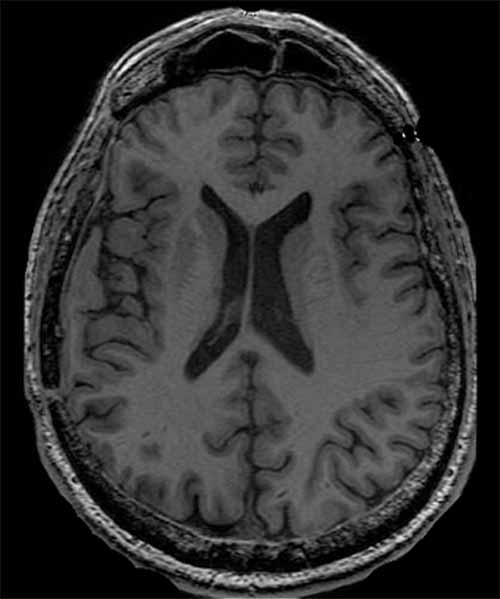
\includegraphics[width=4.5cm]{mri-t1-brain}
  \caption{MRI slice of the brain using $T_1$-weighting \cite{abdulla2025MRI_weighting}.}
  \label{fig:MRI-T1-weighting}
\end{figure}

\section{$T_2$-weighted imaging}
\begin{itemize}
\item The contrast of the images depends on $T_2$.
\end{itemize}
\vspace{-3ex}
\begin{figure}[!b]
  \centering
  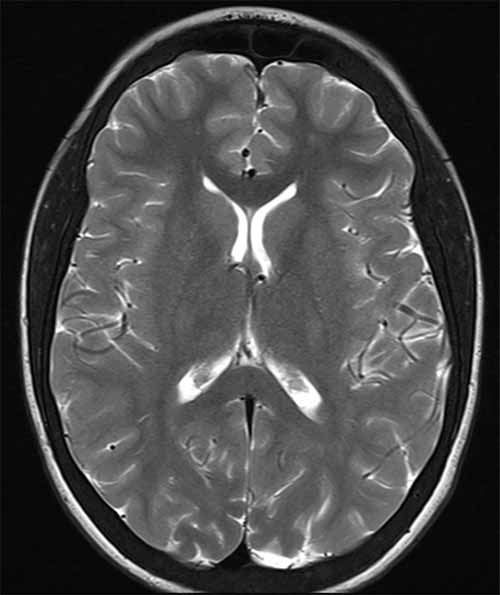
\includegraphics[width=4.5cm]{mri-t2-brain}
  \caption{MRI slice of the brain using $T_2$-weighting \cite{abdulla2025MRI_weighting}.}
  \label{fig:MRI-T2-weighting}
\end{figure}

\section{PD-weighted imaging}
\begin{itemize}
\item The contrast of the images depends on the density of hydrogen
  protons.
\end{itemize}
\vspace{-3ex}
\begin{figure}[!b]
  \centering
  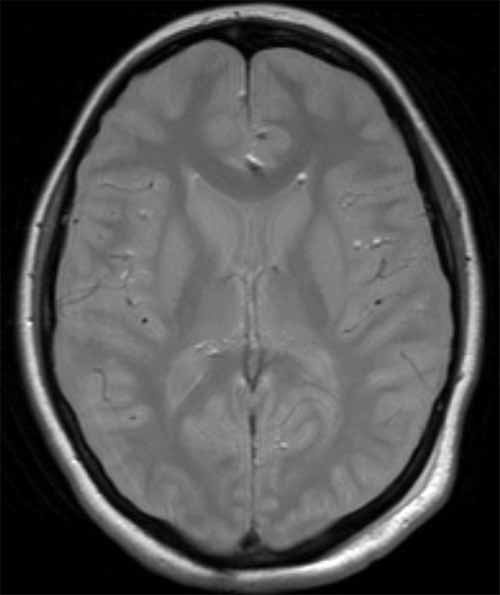
\includegraphics[width=4.5cm]{mri-pd-brain}
  \caption{MRI slice of the brain using PD-weighting \cite{abdulla2025MRI_weighting}.}
  \label{fig:MRI-PD-weighting}
\end{figure}

\section{Spatial encoding}
\label{sec:spatial_encoding}
\begin{itemize}
\item Remember: The hydrogen nuclei resonate at a
  \popup{frequency}{Larmor frequency.} that depends on the strength of
  the magnetic field, $B_0+B_1$, which is a \popup{\gls{RF}
    signal}{$B_0$ is constant but $B_1$ is a time-variying
    signal. Obviously, the sum is also variable over time.}
\item Therefore, modifying $B_0+B_1$ in: (1) amplitude, (2)
  frequency, and (3) phase, we can know the resonating frequency (and
  phase) of a \popup{3D section}{A cuve of tissue.} of the patient.
\end{itemize}
\vspace{-4ex}
\begin{figure}[!b]
  \centering
  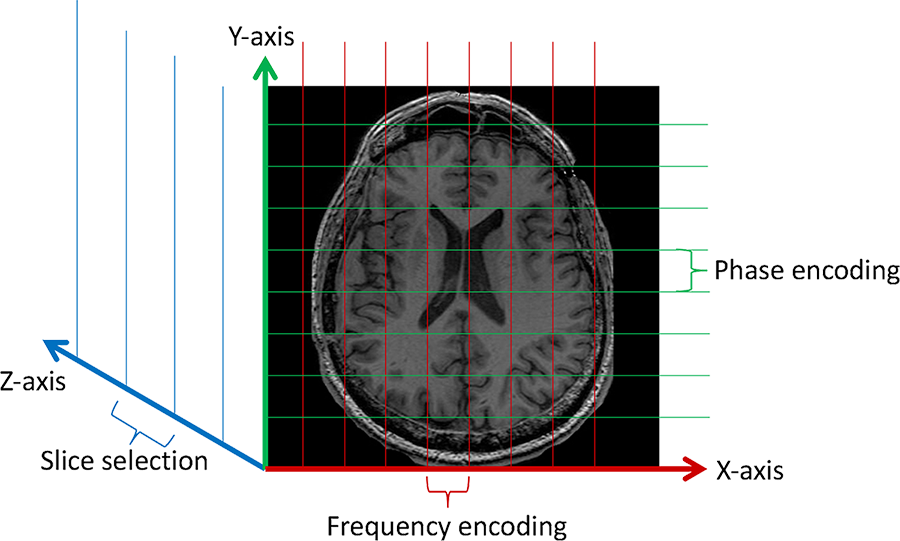
\includegraphics[height=4.0cm]{mri-spatial-localisation}
  \caption{Spatial ``encoding'' \cite{abdulla2025MRI_encoding}.}
  \label{fig:MRI-encoding}
\end{figure}

\begin{itemize}
\item Therefore, using \popup{phase-sensitive band-pass filters}{Also
    called complex filters.}, we can determine the amplitude of the
  signal generated by each 3D section (also known as \gls{FOV}).
\item This information is, by definition, a \popup{coefficient in the
    Fourier domain}{Fourier coefficients are complex numbers, with
    amplitude and plase, or alternatively, real part and imaginary
    part.}.
\item Such information is received by the RF coils that apart from
  generate the gradients in the $XY$-plane, act as a RF antenna.
\end{itemize}

\section{The K-space}
\begin{itemize}
\item In its \popup{simplest version}{The K-space can be also a 3D
    tensor, and the reconstruction can be found using the 3D inverse
    Fourier transform.}, the K-space is a 2D matrix where the
  amplitude and phase of each 3D section of a slice is stored.
\end{itemize}
\vspace{-4ex}
\begin{figure}[!b]
  \centering
  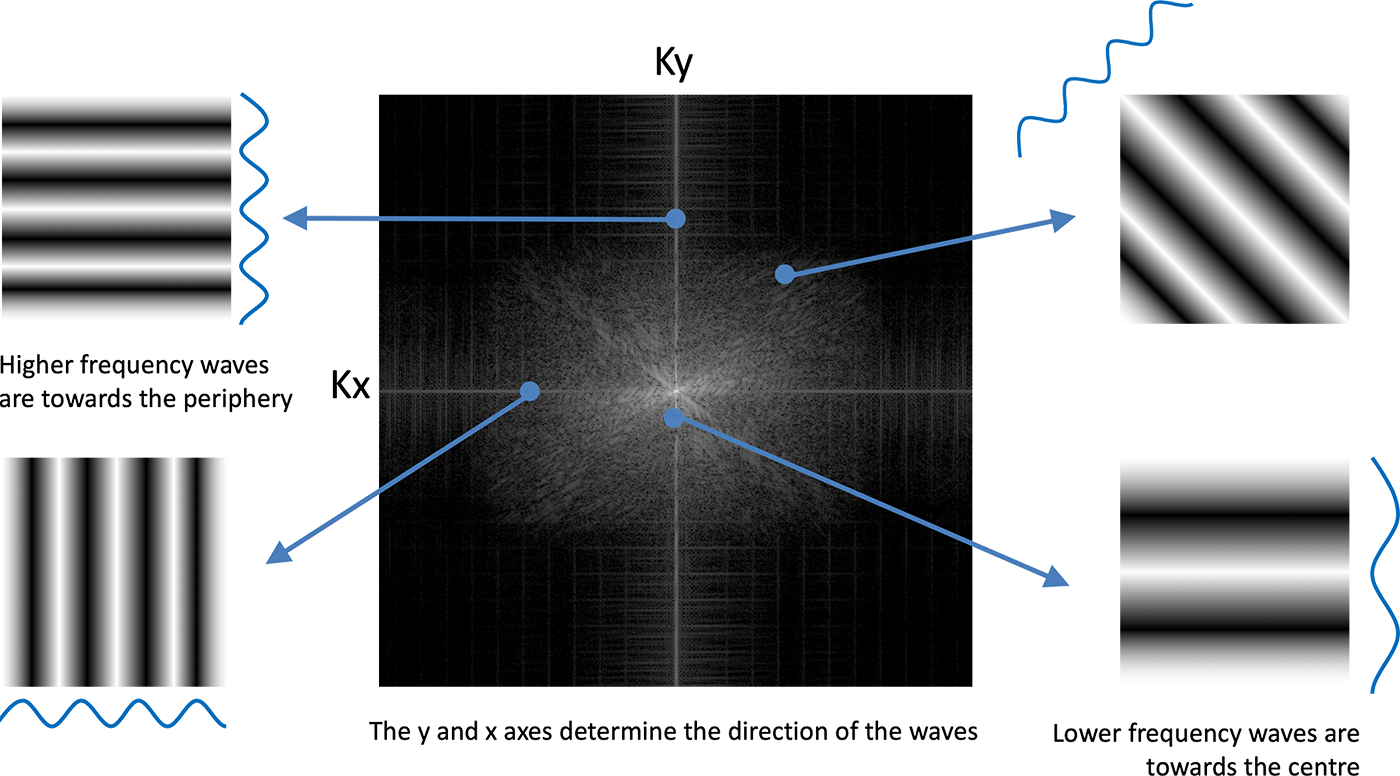
\includegraphics[height=5.5cm]{mri-kspacewavesignal}
  \caption{The K-space and some single-coefficient inverse transformations \cite{abdulla2025MRI_Kspace}.}
  \label{fig:MRI-Kspace}
\end{figure}

\section{3D reconstruction}
\begin{itemize}
\item To reconstruct a slice, we need to compute the 2D inverse
  Fourier transform of the content of the corresponding K-space.
\item To obtain the final 3D reconstruction, all the reconstructed
  (2D) slices are stacked.
\item Notice that in MRI, the tomograms are in the Fourier domain.
\end{itemize}

\section{Image quality in \acrshort{MRI}}
\begin{enumerate}
\item \gls{SNR}: In the case of MRI depends on the strength of the
  signal received by the antenna (precession of coherent
  magnetization), and the strength of noise signal (random frequencies
  existing in space and time, primarily from thermal motion of the
  molecules (in the patient) and background electrical noise of the
  electronics).
\item The SNR increases with the \popup{strength of B0}{As the
    magnetic field strength increases, the Net Magnetic Vector (NMV)
    increases, leading to more available magnetization and
    consequently higher SNR. Doubling the field strength approximately
    doubles the SNR.} \cite{westbrook2018mri}, the \popup{proton
    density}{Areas with a high concentration of MR-active protons
    (e.g., the pelvis) yield higher signal and thus higher SNR,
    whereas areas with low proton density (e.g., the lungs) result in
    lower signal and SNR.} \cite{westbrook2018mri}, the \popup{coil(s)
    efficiency and distance to the sample}{Basically, the SNR is
    proportional to the inverse of the diameter of the tube. The power
    of the excitation RF signals is also proportional to the SNR.},
  the \popup{\emph{signal scanning times}}{Longer TR (Time-Repetition)
    allows for greater longitudinal magnetization recovery, making
    more signal available for conversion to transverse magnetization,
    which typically improves SNR. Shorter TE (Time-Echo) allows less
    coherent transverse magnetization to decay before the echo is
    collected, resulting in higher SNR.} \cite{westbrook2018mri}, the
  \popup{Number of Signal Averages (NSA)}{Increasing the NSA directly
    increases SNR, as correctly encoded signal is reinforced while
    random noise averages out.} \cite{westbrook2018mri}, the
  \popup{size of the voxels}{Larger voxels contain more spins, which
    contribute to a higher signal and consequently increased SNR.}
  \cite{westbrook2018mri}, and reconstruction algorithms
  \cite{bushberg2011essential}.
\item \textbf{Spatial resolution}: Depends fundamentally on the \emph{minimal
    slice-thickness} provided by the internal coils, the
  resolution of the k-space, and on the magnetic field
    strength (B0) to provide a high enought \popup{SNR per voxel}{The SNR
    increases with B0 and the voxel size, so, to increase the
    resolution (decrease the voxel size) we must keep high enough the
    SNR by increasing B0. Otherwise, the noise can make it difficult
    to recognize the pathology}.
\item \textbf{Contrast}: In Magnetic Resonance Imaging (MRI),
    image contrast refers to the differences in signal intensity
    between various anatomical features, between anatomy and
    pathology, or between different tissues. This differentiation is
    crucial for identifying anatomical structures and detecting
    abnormalities within the body \cite{westbrook2018mri}. In the case of MRI data, and considering that the quality
  is a subjective matter, an increase in the contrast (and therefore,
  a higher perceived quality that can help to improve the diagnostic)
  can be obtained if we use \emph{image weighting} (for example,
  T2-weighted volumes usually enhances pathologies), \emph{contrast agents}
  (e.g., gadolinium) can selectively shorten relaxation times,
  increasing the contrast between pathology and normal anatomy, among
  \emph{other MRI contrast-enhancing techniques} (magnetization
  transfer contrast, phase-contrast MR angiography, or the use of
  presaturation pulses) \cite{westbrook2018mri}.
\end{enumerate}
